% CHAPTER 1 LESSON 2
\clearpage
\section{Speech Production}
\label{Speech Production}

Speech production begins with the lungs. The lungs produce the airflow and therefore the energy required to produce speech. This energy then flows through the larynx where the vocal chords are located.  The vocal chords can then begin to vibrate to produce a voiced speech sound or not vibrate to produce an unvoiced speech sound.  This excitation then passes through the vocal tract whose shape can be modified through changes of the tongue, lips, jaw, etc. Each shape corresponds to a different resonance, almost like filling a glass with with different levels of beer to produce different tones.  It is these resonances that produce the different speech sounds that we can then understand.\\
\\
Figure 1, depicts the different parts of the vocal tract that are involved in producing speech. The main two sections are the oral cavity and the nasal cavity. These are separated by a sort of switch called the valluum. The tongue and lips also have important functions in changing the volume of the vocal tract and therefore producing different vocal sounds.\\

\begin{wrapfigure}{r}{0pt}
    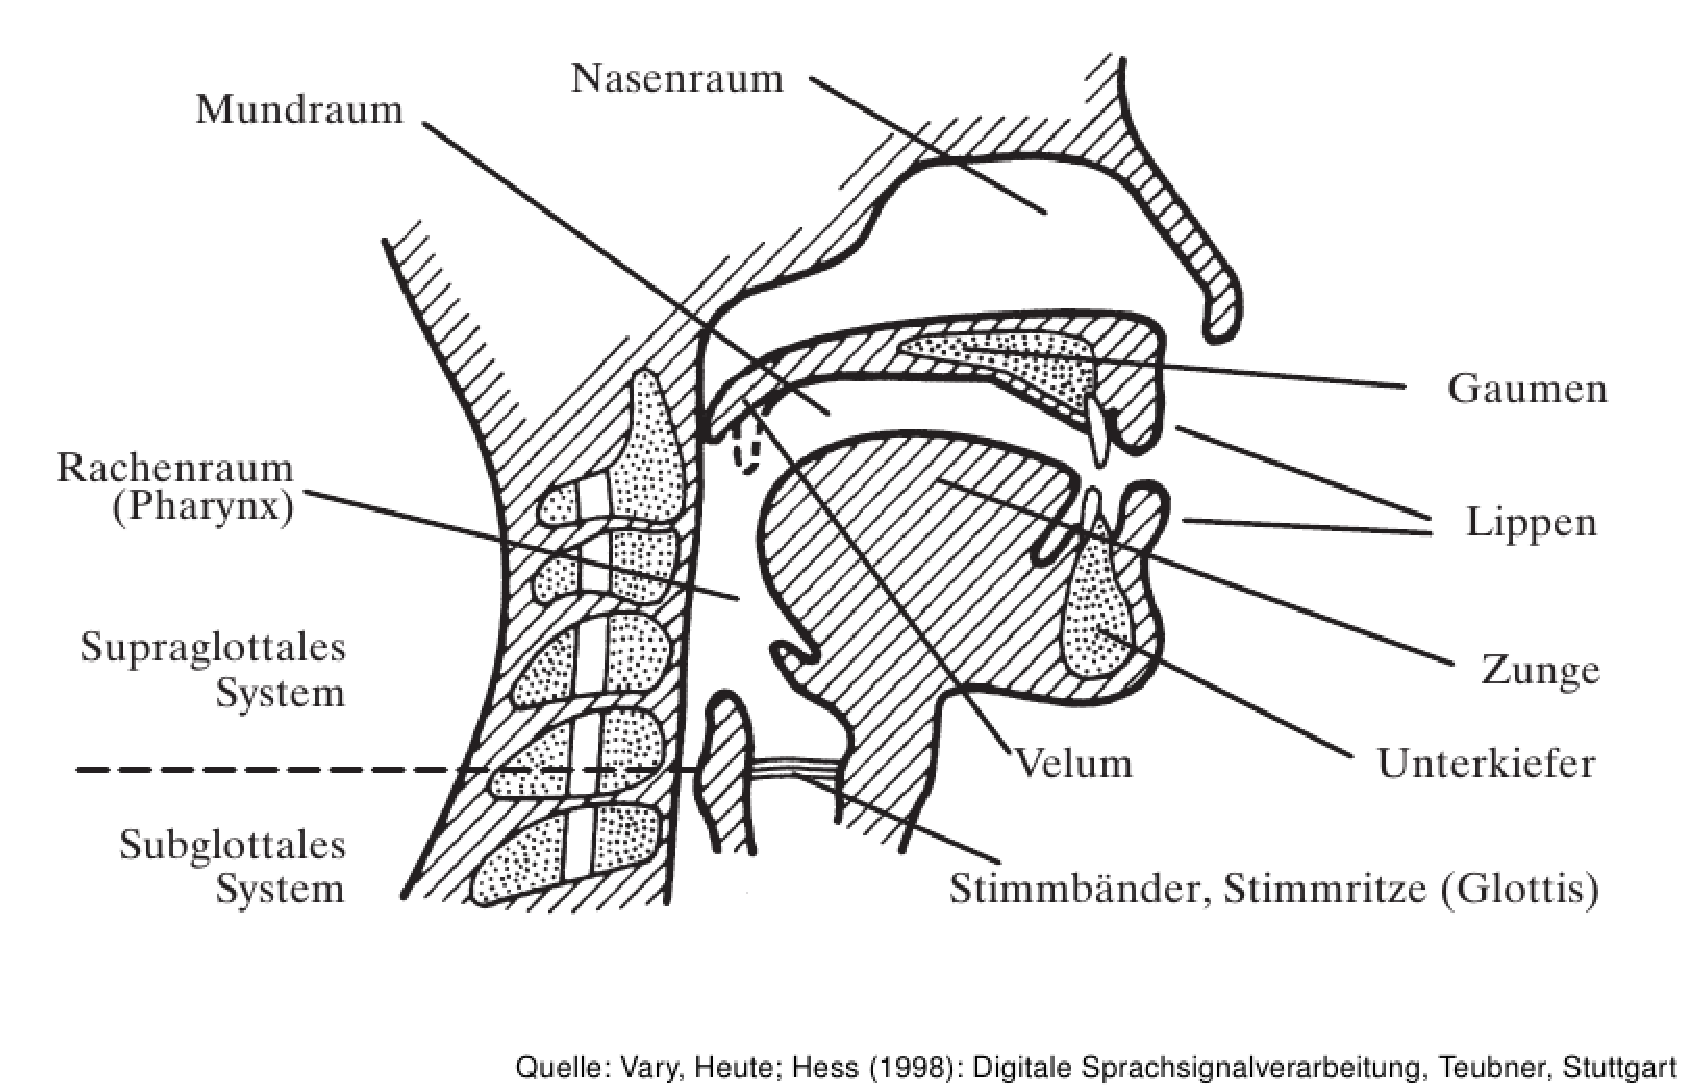
\includegraphics[width=0.7\textwidth]{Pictures/Chapter1_Lesson2/vokaltrakt-eps-converted-to.pdf}
    \caption{The vocal tract.}
\end{wrapfigure}

There are many speech sounds that we can produce and these sounds change for different languages. Probably the most obvious distinction that we can make between all of these vocal sounds is to separate them into voiced and unvoiced. Voiced speech sounds are those produced when our vocal chords vibrate. The best examples are the vowels.  These are sounds where the excitation signals are a periodic vibration of the vocal chords.  There are also unvoiced sounds. These are sounds where the glottus is not vibrating.  These are sounds such as the fricative  /sh/.  Plosives are also unvoiced speech sounds where there is a  complete constriction of the vocal tract and then a sudden opening such as /k/,/p/,/t/.  There are also sounds that are mixture of the two types of excitation such as /v/. \\
\\
Figure 2 shows how these different speech sounds look in the time domain. It was said that a voiced speech sound has a periodic excitation.  This can be seen in the periodic structure in the time domain plot.  The distance between two peaks in the plot is called the fundamental period, or the difference in time between the opening of the glottus. Fig 2b depicts an unvoiced speech signal.  Because there is no periodic excitation of the glottus, the excitation signal is more random in nature. This can be seen by the amount of zero crossings in the time domain plot.  Fig 2c shows a transition between two speech signals.\\

\begin{wrapfigure}{l}{0pt}
    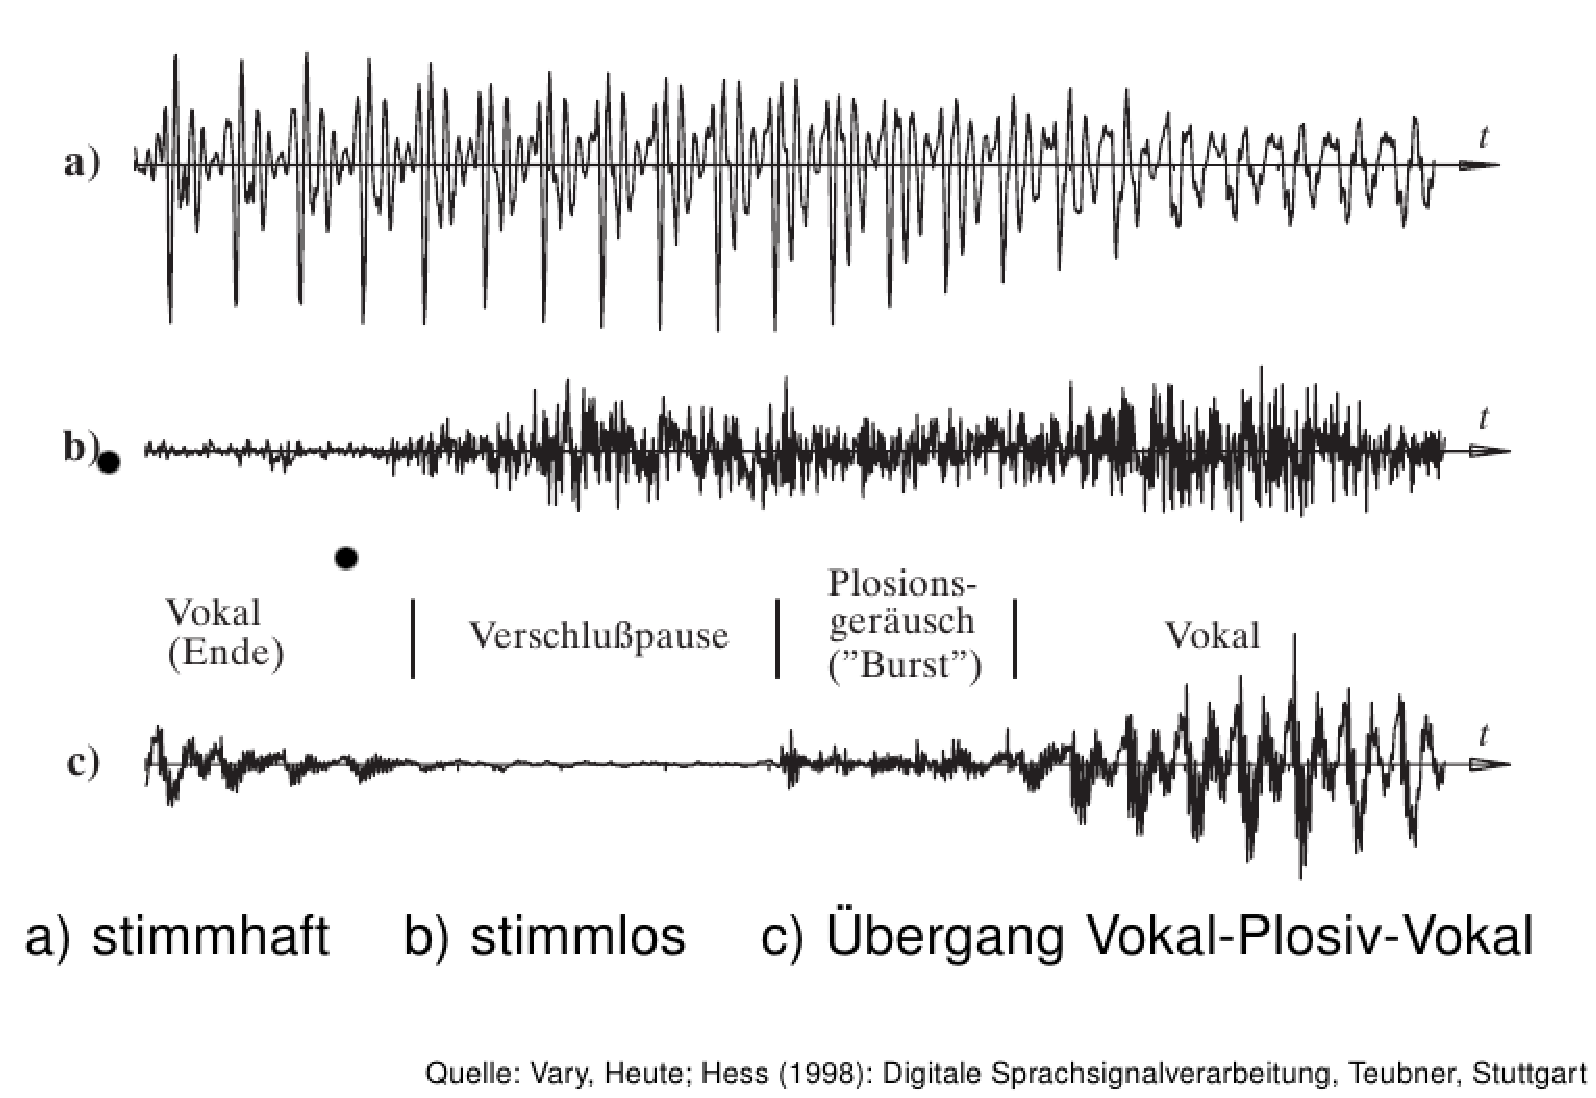
\includegraphics[width=0.7\textwidth]{Pictures/Chapter1_Lesson2/sprachlaute-eps-converted-to.pdf}
    \caption{Time domain signals of voiced and unvoiced speech.}
\end{wrapfigure}

Speech sounds convey meaning and because some of these sounds are different, however still convey the same meaning, there is a system to classify them. A phone is defined as the smallest speech segment with distinct physical or perceptual properties. To call a speech sound a phone is to say that there are no other segments of speech that are the same as that particular segment of speech.  Then there are phonemes.  These are the smallest segments of speech that can change the meaning of a word.  The phoneme consists of a set of phones, so phones are actually different realizations of a phoneme. All of the phones that belong to one phoneme are called allophones. One allophone is one phone of the many that constitute a phoneme. One phoneme can consist of many allophones.  For example, if you take the words ''kiss'' and ''kill'', they have very different meanings, however the difference is only in the phoneme at the end.  This is different with the words  ''cat'',''kit'', ''school'', ''skill''.  These all contain the phoneme /k/ but are pronounced differently due to the different vowel transitions and would, therefore, all be classified as different phones of the same phoneme /k/.\\
\\
Natural human languages have between 10 and 80 phonemes. These can be characterized by the way in which they are articulated, whether they are voiced or unvoiced, and in which place they are articulated.  Place of articulation is basically saying where the tongue is placed in order to produce the speech sound. The different parts of the vocal tract can be used to generate the different phonemes and are also differ across cultures.  The Americans use quite a bit of retroflex, rolling the tongue backwards to create a rolled  ''r' sound. Germans tend to use a glottal stop to distinguish between ''verreisen'' and ''vereisen''. There is a phonetic alphabet that can be used to describe all languages. Fig 3 shows this phonetic alphabet distinguished by place and type of articulation.\\

\begin{wrapfigure}{l}{0pt}
    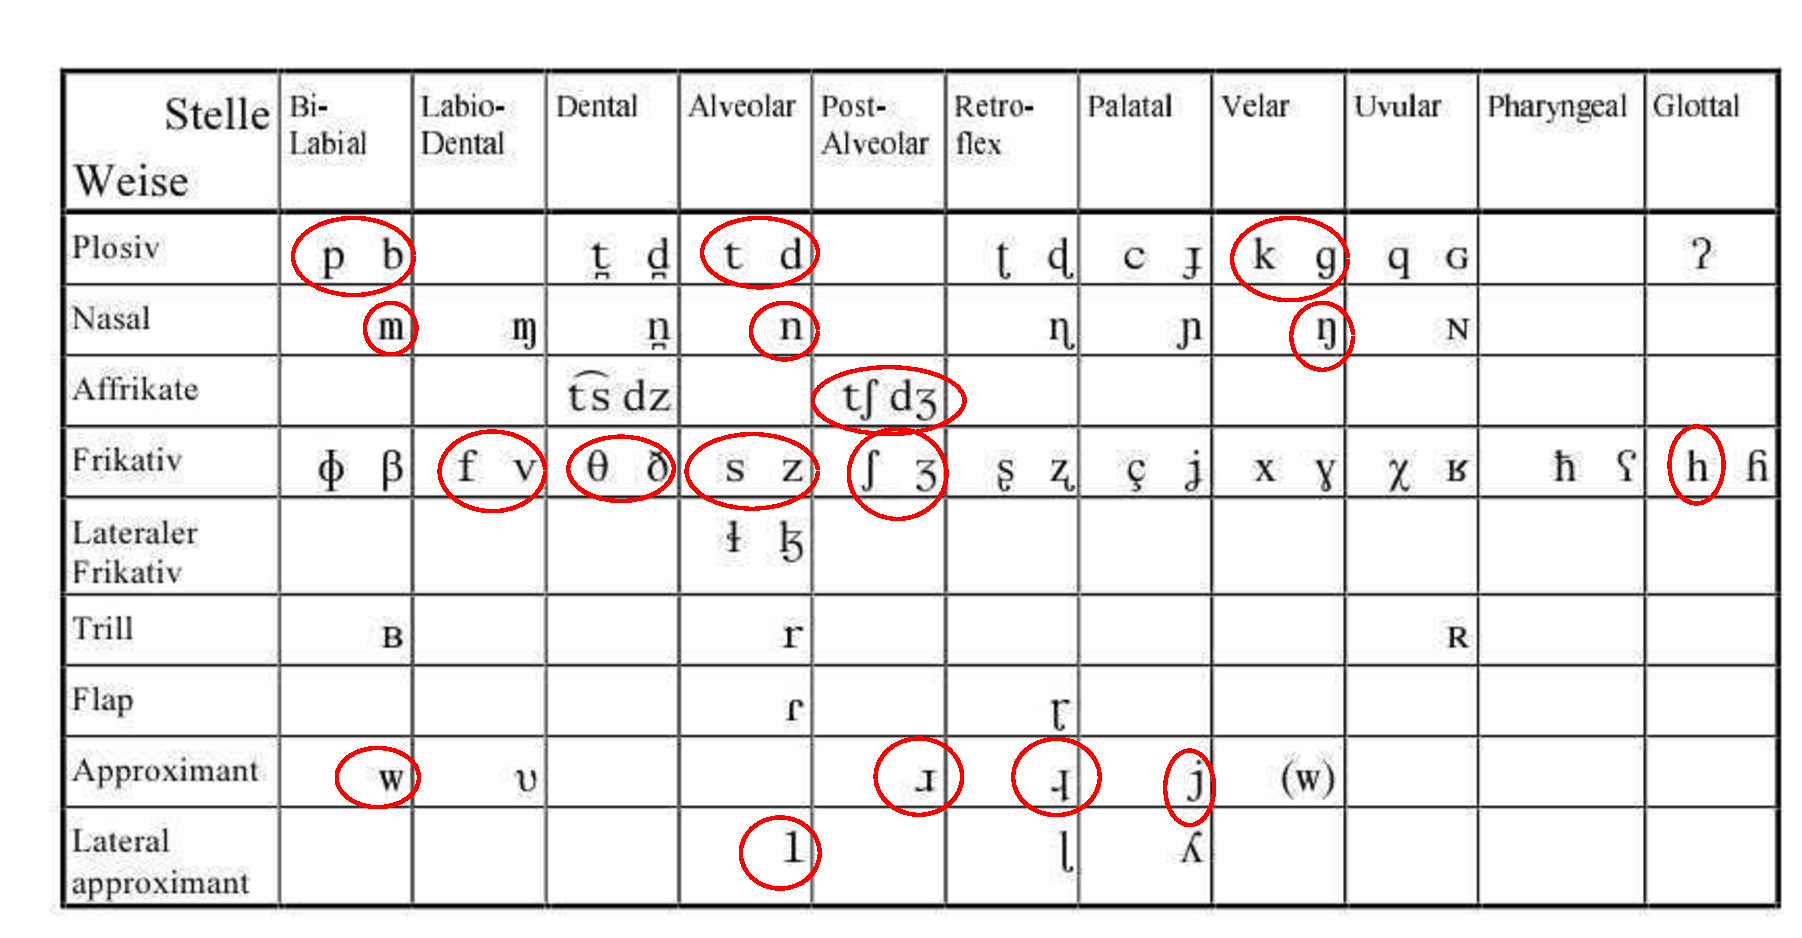
\includegraphics[width=0.7\textwidth]{Pictures/Chapter1_Lesson2/intPhonAlphabet_konsonanten_english2-eps-converted-to.pdf}
    \caption{The phonetic alphabet}
\end{wrapfigure}

Vowels can be distinguished by the position of the tongue in the oral cavity when they are generated.  These are called the cardinal vowels. As with the phonetic alphabet, we are looking for a language independent description. This is done by mapping the position of the tongue in two dimensions, Front to back and high to low, to the vowel sound.  This mapping can then be used to order the corresponding phonemes.  These are called the primary vowels as opposed to the secondary cardinal vowels which are less common and more difficult to say. On one axis, there is the positioning of the tongue from back to front, and then a different axis for the opening of the mouth. It is important to note that the secondary vowels are produced with open lips.\\

Co-articulation is a term used to describe the fact that we produce the same phonemes differently dependent on the content.  This is basically due to the fact that we cannot change our vocal tracts instantly, but there will always be a smooth transition of the tongue from one position to the next.  For instance when you say ''hen'',  it is usually an aveolar sound where the tongue is placed behind the front teeth. However if you say tenth, the /n/ is followed by a /th/, a more dental sound. Therefore, the /n/ will also be pronounced more dentally.  \\

Prosody is another important characteristic of speech.  It is defined as the rhythm, stress, and intonation of speech.  Mostly when people speak of prosody, they speak of the intonation of speech, the melody of the sentence that is said. However, the concept of prosody also encompasses the rhythm and the stress of a speech utterance. Prosody also carries information. It could be the difference between a question and a statement. If we ask a question, we usually raise the fundamental frequency at the end of the sentence.  We also use it to put emphasis on certain words. ''Put the GREEN ball on the table''.  ''Put the green BALL on the table''.  It also carries information about the emotional state of the speaker. For instance, if I yell, then this will usually have a different meaning than if I whisper.  

